\chapter{Seventh chords, edge Tonnetze and non-orientable surfaces}\label{ch:nonorient}

\section{From triads to larger chords}
Four- and five-note chords do not fit on a triangular surface directly. Two strategies appear in the literature.
One raises the dimension: Gollin's three-dimensional Tonnetz places dominant and half-diminished sevenths as
tetrahedra \citep{gollin1998}, and seventh-chord analogues of the $PLR$ group have been studied as groups acting on
the classical seventh-chord types \citep{cannas2017} and through generalized duals of the Tonnetz
\citep{cannas2018}; Boland and Hughston build a tone network for ``Tristan-genus'' chords from a point--line
configuration \citep{boland2025}. The other strategy, adopted in the presentation, \emph{reduces} each chord to
three ``essential'' notes so that chords remain triangles.

\begin{correctionbox}
The ``Edge Tonnetz'' slide reduces C7 = C--E--G--B$\flat$ to C--E--B$\flat$ ``because the dominant note (G) does not
change the way the chord sounds''. The omitted note is the chord's \emph{fifth}; ``dominant'' names a chord
function (V), not a chord member. The fifth is the standard note to omit because the root already implies it
through the overtone series, while the third and seventh define the chord quality. The slide reduces
Cmaj9 = C--E--G--B--D to C--E--D (root, third, ninth). That is a legitimate choice, but it discards the major
seventh, which distinguishes maj9 from the dominant-ninth chord; jazz pianists more often keep third, seventh and
ninth (E--B--D). \code{tonnetzkit.essential\_notes} implements both (\code{"maj9"} and \code{"maj9\_jazz"}).
\end{correctionbox}

With the slide's reductions, the dominant-seventh shell on root $r$ is $\{r,r+4,r+10\}$ and the major-ninth
shell is $\{r,r+2,r+4\}$. Both lie inside the whole-tone scale containing $r$, which is why the presentation
builds a ``Tonnetz based on the whole tone scale''. Its hand-drawn diagram labels triangles with chords (A7, G9,
F7, \dots) and \emph{edges} with notes: in an edge Tonnetz, notes are edges rather than vertices.

\section{Reconstructing the slide: a triangulated projective plane}
The diagram on the slide ``Now how does the surface look?'' is a hexagonal region of side 2 in the triangular
lattice: 24 triangles, 19 vertices and 42 edges before gluing. The thick arrows around its border indicate that
each boundary point is glued to the \emph{antipodal} boundary point, the point diametrically opposite. After gluing,
the 12 boundary vertices become 6 and the 12 boundary edges become 6, so
\[
V=7+6=13,\qquad E=30+6=36,\qquad F=24,\qquad \chi=13-36+24=1,
\]
matching the slide's ``$V-E+F=1$''. \Cref{fig:rp2} shows the construction.

\begin{figure}[t]\centering
\begin{minipage}{0.46\linewidth}\centering
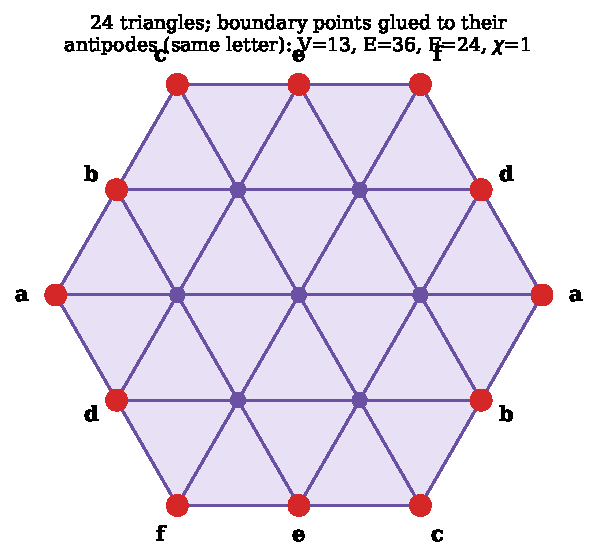
\includegraphics[width=\linewidth]{figures/rp2_hexagon.pdf}
\end{minipage}\hfill
\begin{minipage}{0.5\linewidth}
\caption{The slide's surface, reconstructed: a hexagonal patch of 24 triangles whose boundary vertices with the same
letter (and the boundary edges between them) are identified antipodally. A disc with antipodal boundary points
identified is, by definition, the real projective plane.}\label{fig:rp2}
\end{minipage}
\end{figure}

\begin{proposition}\label{prop:rp2}
The glued hexagon is a triangulation of the real projective plane $\mathbb{RP}^2$. Its Betti numbers are
$(1,0,0)$ over $\QQ$ and $(1,1,1)$ over $\Z_2$, and it admits no coherent orientation.
\end{proposition}
\begin{proof}
A closed disc with antipodal boundary identification is a standard model of $\mathbb{RP}^2$. Independently:
every edge lies in two triangles and every vertex link is a single cycle, so the complex is a closed surface;
the orientation-propagation test fails; and by \cref{thm:classification}, $\chi=1$ with non-orientability gives
$k=1$ cross-cap. The Betti numbers are computed by \code{SimplicialComplex.betti}; the difference between the two
fields reflects $H_1(\mathbb{RP}^2;\Z)=\Z_2$.
\end{proof}

The slide's own reasoning is also correct and worth making explicit: if the surface were orientable, then
$2-2g=1$ would force $g=\tfrac12$, which is impossible. The surface therefore \emph{must} be non-orientable,
which is exactly why the next slide turns to M\"obius strips, Klein bottles and Boy's surface (an immersion of
$\mathbb{RP}^2$ in 3-space).

\section{The pitch-class complex tells a different story}
It is instructive to compare the diagram with the chord complex of Chapter~\ref{ch:topology}, where notes are
vertices. Inside one whole-tone scale (6 notes) there are 6 dominant-seventh shells and 6 major-ninth shells:
\begin{center}\small
\begin{tabular}{@{}lccccl@{}}\toprule
Triangles & $V$ & $E$ & $F$ & $\chi$ & Space\\\midrule
6 dom.-seventh shells $\{r,r{+}4,r{+}10\}$ & 6 & 15 & 6 & $-3$ & orientable, with boundary\\
6 major-ninth shells $\{r,r{+}2,r{+}4\}$ & 6 & 12 & 6 & 0 & cylinder\\
both (12 chords) & 6 & 15 & 12 & 3 & not a surface (see text)\\\bottomrule
\end{tabular}
\end{center}
The combined complex has Betti numbers $(1,0,2)$ and is not a surface at all. Hence the projective plane of the
slide is not the vertex-based chord complex; it is one particular \emph{edge-labelled} gluing, and the choice of
gluing matters. The next section quantifies how much.

\section{Edge-labelled gluings: a census}
\begin{definition}
Given a list of chords, each a triangle whose three edges carry its three notes, an \emph{edge Tonnetz} is obtained
by gluing all edges in pairs, only ever gluing two edges with the same note label, with one of the two possible
orientations for each glued pair.
\end{definition}
Gluing polygons edge-to-edge in pairs always produces a closed surface (possibly disconnected); this is the setting
of the classification theorem. For the 12 shell chords of the whole-tone scale $\{1,3,5,7,9,11\}$ every note
belongs to exactly 6 chords, so each note labels 6 edge slots that must be paired into 3 glued edges: $15$ perfect
matchings times $2^3$ orientations per note, i.e.\ $120^6\approx3\times10^{12}$ gluings. Every one has $F=12$ and
$E=18$, hence $\chi=V-6$, but the number of vertices depends on the gluing.

\begin{figure}[t]\centering
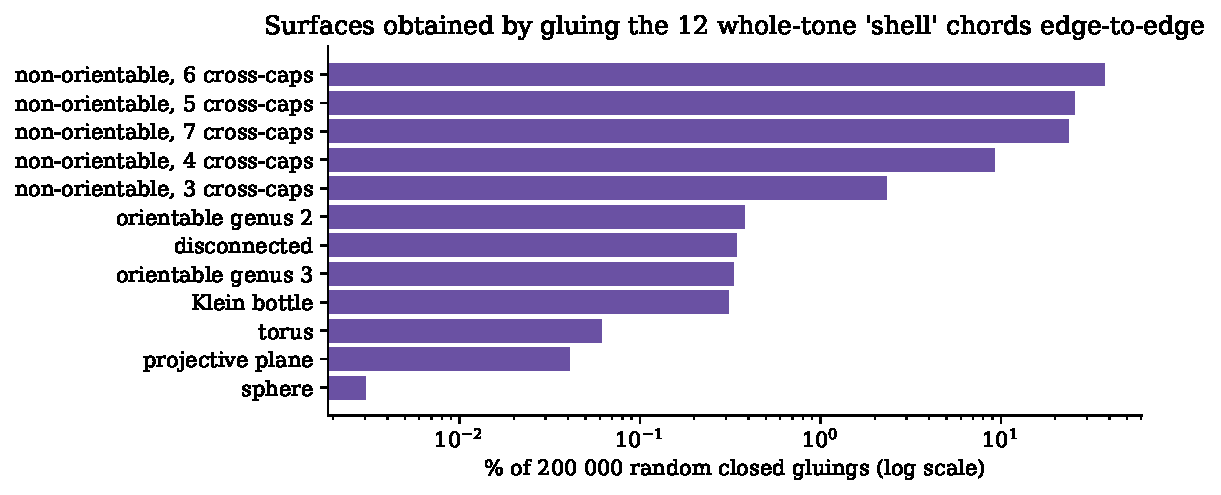
\includegraphics[width=0.86\linewidth]{figures/edge_census.pdf}
\caption{Surfaces obtained from 200\,000 uniformly random closed gluings of the 12 whole-tone shell chords.}
\label{fig:census}
\end{figure}

\Cref{fig:census} shows a Monte-Carlo census of 200\,000 random gluings (\code{sample\_edge\_tonnetze}). The typical
outcome is a non-orientable surface with 5 to 7 cross-caps (together 87\%). Orientable surfaces are rare (0.78\% in
total: genus 2, genus 3, torus, and sphere). The projective plane occurs in only 0.041\% of gluings, and the sphere in 0.003\%.
The surface of the slide is therefore a very special member of a very large family. Two lessons follow.
\begin{enumerate}
\item An edge Tonnetz is not determined by its chord vocabulary alone. A musically motivated gluing rule (for
instance, glue two chords along a note only if they also share a second note, so that adjacent triangles are
parsimoniously related) is needed to make the construction canonical.
\item Finding the gluings with the \emph{largest} Euler characteristic is a combinatorial optimisation problem;
we pose exact enumeration up to symmetry as an open problem in Chapter~\ref{ch:outlook}.
\end{enumerate}

\section{Non-orientable spaces elsewhere in music theory}
Non-orientability is not an exotic accident. The space of unordered two-note chords is a M\"obius band
\citep{callender2008,tymoczko2011}: it is the space of unordered pairs of points on the pitch-class circle, whose
single boundary circle consists of the unisons, and in which the tritones form the central circle of the band. Catanzaro's harmonic strip is a M\"obius band in odd temperaments (Chapter~\ref{ch:topology}), and his
tritone Tonnetze relate to Peck's Klein-bottle Tonnetz \citep{catanzaro2011}. These examples show that the
orientable torus of the classical Tonnetz is a special case, not the norm.

\begin{notebookbox}
\sheet{06\_edge\_tonnetz.ipynb}: rebuild the glued hexagon and verify \cref{prop:rp2}, compute the pitch-class
complexes above, run the census, and search for a spherical gluing.
\end{notebookbox}

\begin{qa}
\Qu{In C7 = C--E--G--B$\flat$, which note is usually omitted in a shell voicing, and why?}
\A{The fifth, G: it adds little to the chord's identity, which is carried by the third (quality) and the seventh
(dominant function).}
\Qu{Verify the counts $V=13$, $E=36$ for the glued hexagon.}
\A{Before gluing: 19 vertices (7 interior, 12 boundary) and 42 edges (30 interior, 12 boundary). Antipodal gluing
halves the boundary: $7+6=13$ vertices and $30+6=36$ edges.}
\Qu{Why must a closed surface with $\chi=1$ be non-orientable?}
\A{Orientable closed surfaces have $\chi=2-2g$, always even.}
\Qu{What are the Betti numbers of $\mathbb{RP}^2$ over $\QQ$ and over $\Z_2$?}
\A{$(1,0,0)$ over $\QQ$ and $(1,1,1)$ over $\Z_2$.}
\Qu{For the 12-chord edge Tonnetz, how many vertices does a spherical gluing have?}
\A{$\chi=V-18+12=2$ gives $V=8$.}
\Qu{Why is the whole-tone pitch-class complex with both chord types not a surface?}
\A{Each whole-tone edge $\{x,x+2\}$ lies in two major-ninth shells and one dominant-seventh shell: three
triangles, whereas a surface allows at most two.}
\end{qa}
